\documentclass{standalone}
\usepackage{tikz}

\begin{document}
    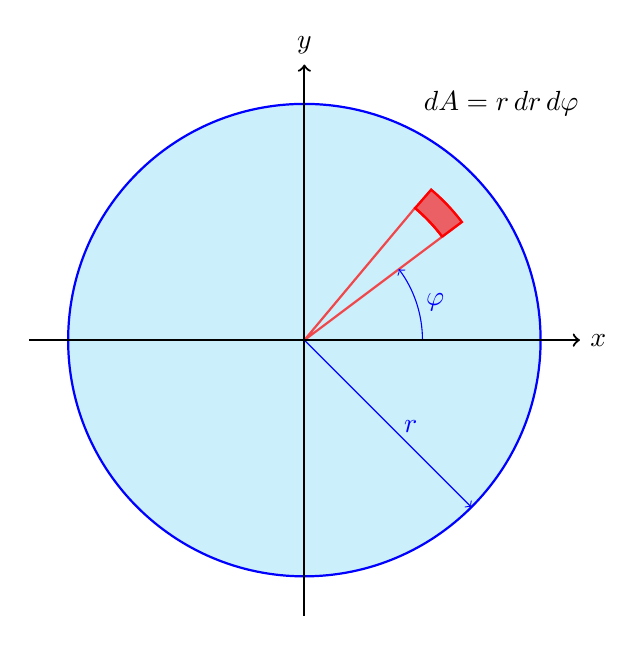
\begin{tikzpicture}
        \pgfmathsetmacro{\step}{0.025}
        
        % Draw the circle
        \fill[cyan, opacity=0.2] (0,0) circle (3);
        \draw[blue, thick] (0,0) circle (3);
%        \foreach \radi in {0,\step,...,3}{
%%            \draw[cyan,line width=3pt,opacity=0.06] (0,0) circle (\radi);
%            \draw[cyan,thin,opacity=0.25] (0,0) circle (\radi);
%        }
        
        % Draw the differential area
%        \draw[red, thick] (1.75,1.313) -- (2,1.51);
%        \draw[red, thick] (2,1.5) arc[start angle=37, end angle=50, radius=2.57cm];
%        \draw[red, thick] (1.75,1.313) arc[start angle=37, end angle=50, radius=2.15cm];
%        \draw[red, thick] (1.406,1.676) -- (1.607,1.91511);
%        \draw[red, thick] (0,0) -- (1.406,1.676);
%        \draw[red, thick] (0,0) -- (1.75,1.313);
        \draw[red,thick,opacity=0.7] (0,0) -- (1.75,1.313) -- (1.75,1.313) arc[start angle=37, end angle=50, radius=2.22cm] -- (0,0);
        \draw[red,thick] (1.75,1.313) -- (2,1.5) -- (2,1.5) arc[start angle=37, end angle=50, radius=2.5cm] -- (1.406,1.676) -- (1.406,1.676) arc[start angle=50, end angle=37, radius=2.22cm];
        \draw[red,thick,fill=red,opacity=0.6] (1.75,1.313) -- (2,1.5) -- (2,1.5) arc[start angle=37, end angle=50, radius=2.5cm] -- (1.406,1.676) -- (1.406,1.676) arc[start angle=50, end angle=37, radius=2.22cm];
        
        % Draw the radial line and arc for the angle
        \draw[->, blue] (0,0) -- (2.12132,-2.12132) node[above] at (1.35,-1.3) {$r$};
        \draw[->, blue] (1.5,0) arc[start angle=0, end angle=37, radius=1.5] node[midway, right] {$\varphi$};
        
        % Draw the small rectangle indicating the angle
%        \draw[thick] (1.1,0) -- (1.1,0.25) -- (1,0.25);
        
        
        % Draw the axes
        \draw[->, thick] (-3.5,0) -- (3.5,0) node[right] {$x$};
        \draw[->, thick] (0,-3.5) -- (0,3.5) node[above] {$y$};
        
        % Add the text for the differential area element
        \node at (2.5, 3) {$dA = r \, dr \, d\varphi$};
        
    \end{tikzpicture}
\end{document}
